\documentclass[14pt,hyperref={CJKbookmarks=true}]{beamer} %14pt为字体尺寸,默认值11pt.有8-12;14;17;20;bigger;smaller
\usepackage[space,noindent]{ctex}
\usepackage{xcolor}
\usepackage{animate}
\usetheme{Boadilla}   %蓝色主题
%\logo{\includegraphics[scale=0.15]{logo.jpg}}  %校徽的logo,可有可无,目前还没有找到使校徽置于右上方的办法
%\setbeamercolor{normal text}{bg=black!10}
\usecolortheme{whale} %颜色主题为
%\usetheme{Berkeley}  %演示主题为侧边导航条
\usetheme{default}    %默认主题
\renewcommand{\tablename}{表}
\begin{document}
	\newtheorem{THeorem}{定理}  %自定义定理
	\newtheorem{DEfinition}{定义} %自定义定义
	\newtheorem{PRoof}{证明}  %自定义证明
	%\theoremstyle{plain}  %定理的格式有example,plain,definition三种,默认值为plain
	\theoremstyle{example}
	%\theoremstyle{definition}
	\newtheorem{EXample}{示例}  %自定义例子
	\kaishu
	\setbeamertemplate{theorems}[numbered]  %给定理类模块的标题添加序号,如果幻灯片里定理类数学表达式不多就可以取消该命令。
	\title{你的标题}
	\author{$\rho$爱上$\theta$}
	\institute[你的院系全称]{所属院系简称}
	\date{\today}
	\begin{frame}
		\titlepage
	\end{frame}
	\section{概述}
	\subsection{基本理论}
	\begin{frame}{帧标题}{副标题}
		基本理论的要点1、2、3...
	\end{frame}
	\section{研究方法}
	\begin{frame}{研究方法}
		研究和研究方法简介
	\end{frame}
	\subsection{主要论点和论据}
	\begin{frame}{主要论点和论据}
		根据计算机模拟和试验
	\end{frame}
	\section{总结}
	\subsection{研究意义与创新点}
	\begin{frame}{总结}
		通过大量研究表明
	\end{frame}
	\begin{frame}{定理类模块}
		\begin{DEfinition}
			有一个角是直角的三角形是直角三角形。
		\end{DEfinition}
		\begin{THeorem}
			直角三角形斜边的平方等于另外两个边平方之和。
		\end{THeorem}
		\begin{PRoof}
			画一条通过点$A$和点$B$的线段$a$。\dots \\
			这就证明了\dots.    %在proof模块里面已经有了证毕符号,不用再写\qed,但是在自定义的EXample中,就得加上它才可以。
		\end{PRoof}
		\begin{EXample}
			$x^{3}+2x^{2}+x+1=0$
		\end{EXample}
	\end{frame}
	\begin{frame}{三种色调的文本模块}
		这三类文本标题可以有作者自行设置,并以不同的背景颜色来区别其文本的性质。其中标题这个参数是必须要有的,具体可见P449页。
		\begin{block}{基本性质}
			$\frac{a}{b}=\frac{am}{bm}$
		\end{block}
		\begin{exampleblock}{举例模块}
			$\frac{a}{b}\cdot\frac{c}{d}=\frac{ac}{bd}$
		\end{exampleblock}
		\begin{alertblock}{\heiti 注意!}
			在分式中,分母不能为零。
		\end{alertblock}
	\end{frame}
	\begin{frame}{彩色盒子}\setbeamercolor{mycolor}{fg=black,bg=pink}%自定义一个名为Mycolor的beamer颜色,其前景是黑色,背景为粉红色
		如果正整数$ x,y,z $能够满足下列不定方程:\\
		\centerline{\begin{beamercolorbox}[rounded=true,shadow=true,wd=26mm]{mycolor}
				$ x^2+y^2=z^2 $   %行距中命令\centerline是TEX拓展命令,latex的居中命令\centering和居中环境center在彩色盒子不起作用。
		\end{beamercolorbox}}则它们叫做勾股数。\\[20pt]
		圆周率
		\hspace{2pt}\raisebox{-2mm}{%
			\begin{beamercolorbox}[rounded=true,shadow=true,wd=19mm]{mycolor}
				$ \pi=3.14 $
		\end{beamercolorbox}}\hspace{3pt}
		是圆周与直径之比。
	\end{frame}
	\begin{frame}{圆角盒子}
		在1673年,法国数学家费马提出:
		\setbeamercolor{myupcol}{fg=white,bg=purple}
		\setbeamercolor{mylowcol}{fg=black,bg=pink}
		\begin{beamerboxesrounded}[upper=myupcol,lower=mylowcol,shadow=true]{费马猜想}
			当$ n $是一个大于2的整数时,则\\
			\centerline{$ x^{n}+y^{n}=z^{n} $}\\
			这个不定方程没有正整数解。\\
		\end{beamerboxesrounded}
		1995年英国数学家怀尔斯用反证法证明飞马猜想完全可以成立。在这个例子中,分别定义了myupcol和mylowcol两个beamer颜色。
	\end{frame}
	\begin{frame}{列表的应用举例}
		\begin{block}{开普勒定律}
			\begin{enumerate}
				\item  行星绕太阳运动的轨迹是以太阳为焦点的椭圆。
				\pause
				\item  行星与太阳的连线在相等的时间扫过相同的面积
				\pause
				\item  不同行星在其轨道上公转周期的平方与轨道半长径的立方成正比。
			\end{enumerate}
		\end{block}
	利用pause命令可以暂停命令,会产生三张幻灯片
	\end{frame}
\begin{frame}{表格}
	\begin{table}
	\caption{各种移动通信的比较}
	\begin{tabular}{|c|c|c|c|}
		\hline
		           & 2G         & 2.5G     & 3G  \\   \hline
		信号类型    & 模拟        & 数字      & 数字  \\  \hline \onslide<2->
		交换方式    & 分组交换    & 电路交换   & 分组交换\\  \hline  \onslide<3->
		提供服务    & 短信        & 网络      & 多媒体  \\   \hline  \onslide<4->
		传输速率    & 14          & 144       & 2000  \\     \hline
	\end{tabular}
	\end{table}
加入onslide<>命令可以将表格改变为逐行显示。
\end{frame}
\begin{frame}{将一帧分为两栏}
	\texttt{columns}环境可以将一帧分成多栏,通常为两栏,这样便于在插图旁边放置说明文字。
	\begin{columns}[onlytextwidth]  %onlytextwidth相当于将各栏所占据的总宽度设置为totalwidth=\textwidth
		\begin{column}{0.55\textwidth}
			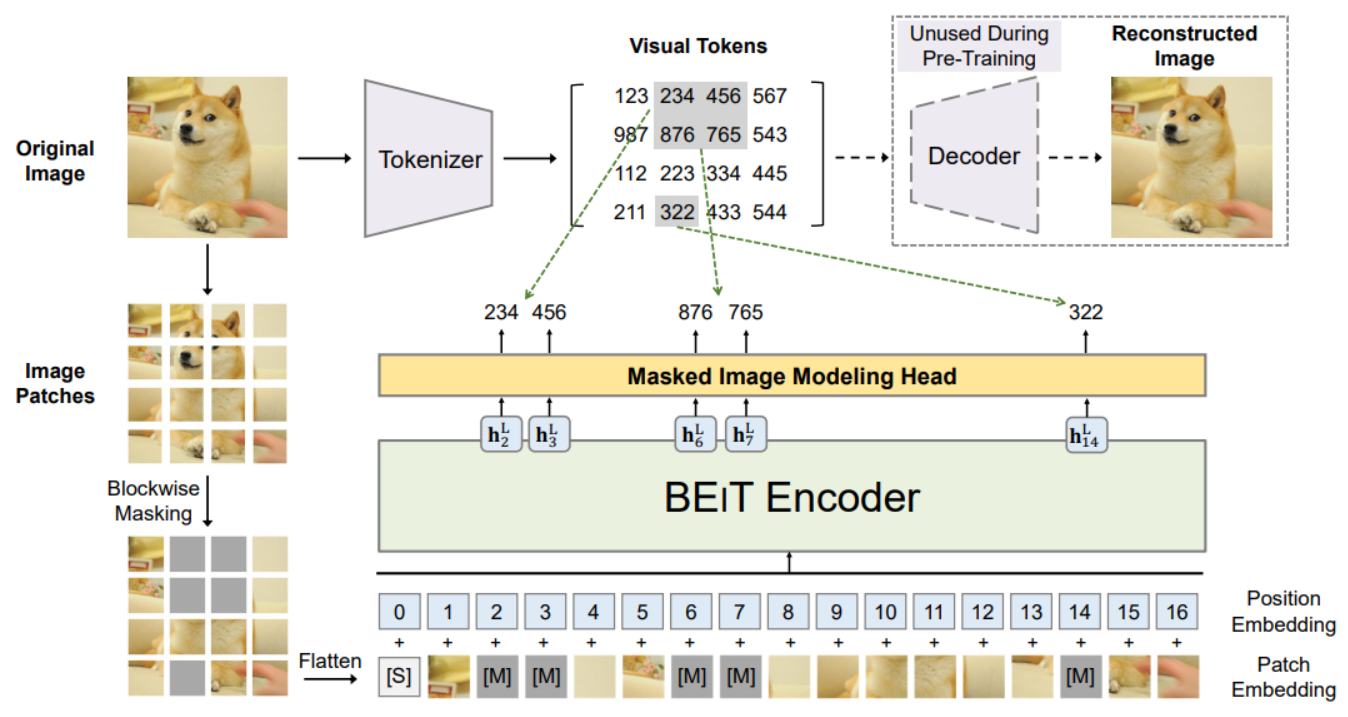
\includegraphics[width=\columnwidth]{"../src/BEiT.png"}
		\end{column}
	\begin{column}{0.45\textwidth}
		左图是蒙特卡洛算法的模拟情况,其中:
		\begin{itemize}
			\item  绿色为圆柱体上下底面的曲线
			\item  蓝色为圆柱体内的随机点
			\item  红色为函数曲面的随机点
		\end{itemize}
	\end{column}
	\end{columns}
\end{frame}
\begin{frame}{参考文献}
\begin{thebibliography}{10}
	
\end{thebibliography}
\end{frame}
\end{document}